\section{Dosímetro Active Pixel Sensor}
\fig{aps}{esquematicos/aps.pdf}{Esquemático del dosímetro APS}
El dosímetro APS tiene una estructura similar a un pixel del sensor de imagen
en una cámara digital. 
Su principio de funcionamiento es medir la carga generada por radiación en la zona desierta de
una juntura p-n.
Hay un nodo flotante del circuito que acumula esta carga,
conectado al cátodo del diodo (\figref{fig:aps}).
Antes de cada medición, se reinicia el circuito llevando este nodo a 
V$_{\text{DD}}$ mediante el transistor de reset M1.
La radiación que incide en la zona desierta de D1 interactúa con la red de
silicio, depositando energía a través de distintos procesos como scattering e
ionización (ver sección~\ref{sec:radiacion}).
Los fotones y electrones secundarios resultantes producen pares electrón-hueco,
que son arrastrados en direcciones opuestas por el campo eléctrico.
Los electrones se acumulan en el cátodo, descargándolo.
Luego de irradiar,
se mide su tensión a través de un par de seguidores M2 y M3.
Los mismos evitan que la medición de tensión modifique la carga en el nodo y
afecte al valor medido.
\subsection{Proceso de fabricación}
Fabricamos tanto el FG como el APS en el proceso XC06 de la empresa X-FAB
\cite{x-fab_0.6_2008}.
El mismo tiene una escala de \SI{0.6}{\micro\meter} y está diseñado para
tensiones de hasta \SI{5}{\volt}.
En su versión estándar, 
cuenta con 1 capa de polisilicio y 2 de metalización.
\subsection{Reset}
Cargamos el nodo flotante a través del drain de un MOSFET de canal P,
con el source conectado a \vdd.
Durante la irradiación llevamos su gate a \vdd, apagándolo.
Para resetear 
llevamos su gate a tierra.
Esto lo coloca en saturación,
cargando la juntura a corriente constante 
y aumentando $V_D$ linealmente hasta $V_t$.
Entonces entra en triodo y va reduciendo la corriente,
cargando asintóticamente hasta \vdd.
Esto permite llevarlo a $V_{dd}$,
mientras que una llave de tipo N sólo llegaría hasta $V_{dd}-V_{tn}$ antes de
apagarse.

El transistor de reset es de área mínima,
para que aporte la menor capacidad parásita posible al nodo flotante.
\subsection{Respuesta a partículas}
Cada partícula deposita una energía promedio que depende de su energía
cinética inicial\cite{berger_response_1969} (ver sección~\ref{montecarloaps}).
Una parte $E$ de esta energía se usa en la creación de pares electrón-hueco,
generando carga 
\begin{align*}
    Q &= \frac{qE}{E_i}
\end{align*}
con $q$ la carga del electrón y $E_i$ la energía de creación de pares,
\SI{3.62}{\electronvolt} en Si.
Esta carga aparece con signo negativo en el cátodo, descargándolo.
Su cambio de tensión
\begin{align*}
    \Delta V &= \frac{Q}{C}
\end{align*}
depende de la capacidad total del nodo $C$.
La misma tiene contribuciones de
\begin{itemize}
    \item juntura de D1,
    \item juntura Drain-Body de M1,
    \item Gate de M2, y
    \item conductores cercanos al nodo.
\end{itemize}
Estas capacidades pueden estimarse a partir de las especificaciones del 
proceso de fabricación,
que indican capacidad por unidad de área y por unidad de perímetro.
Para eso usamos herramientas de EDA (electronic design automation)
que realizan esta estimación automáticamente a partir de la geometría del
diseño (ver sección~\ref{section:diseno_aps}).
\subsection{Cálculos Monte-Carlo}
\label{montecarloaps}
El dosímetro APS detecta energía depositada 
en una región específica de un circuito integrado.
A fines de simularlo, 
simplificamos la geometría del die a tres regiones:
una superficie de SiO$_2$, un sustrato de Si 
y una zona sensible también de Si (\figref{fig:corteaps}).
\fig{corteaps}{figuras/aps/corte.pdf}
{Corte de la geometría usada para simular el APS en Geant4 (no a escala).}
Las dimensiones se extrajeron del diseño del APS 
y de las especificaciones del proceso de fabricación del chip.

Dado que el uso principal de Geant4 es en física de altas energías,
su configuración por defecto no permite simular electrones secundarios por
debajo de \SI{250}{\electronvolt}.
% DETAIL rango a 250eV ~ nm, qué me importa?
Para obtener precisión a escalas de distancia más chicas,
empleamos una lista de procesos compilada para simulaciones en
microelectrónica \cite{Raine201497}.
La misma simula con fidelidad electrones hasta \SI{16.7}{\electronvolt},
cuyo rango en Si es del orden de \SI{0.1}{\nano\meter}.

% FIXME falta este gráfico usando
% ../tesis/figuras/aps/deposicion1electron001.pdf y demás
Los resultados se encuentran en la \figref{fig:energia1electron}.
Se ve que los electrones menos energéticos tienden a frenarse por completo en
el detector, depositando toda su energía.
Los más energéticos, en cambio, depositan una fracción variable de su energía
total.
La energía depositada promedio se encuentra en la
\figref{fig:energiadepositadaaps}.
\fig{energiadepositadaaps}{../poster2015/aps_respuesta.pdf}
{Respuesta promedio a un electrón incidente,
en función de su energía inicial.
Se ve que los electrones menos energéticos se frenan completamente en el
detector.}
\subsection{Fuentes de ruido}
El APS se maneja con corrientes y variaciones de carga y tensión muy
pequeñas.
Por eso es crítico conocer los procesos que introducen ruido y su magnitud.
\subsubsection{Corriente de fuga de juntura p-n}
Al polarizar una juntura p-n en inversa, fluye una corriente de
pérdida\cite{sze_physics_2007} dada por
\begin{align*}
    I&=I_s(e^{\frac{qV}{\eta kT}}-1)
\end{align*}
con $V<0$ la tensión aplicada y $I_s$ y $\eta$ parámetros de fabricación de la
juntura.
El valor de $I$ fluctúa debido a la naturaleza discreta de los portadores que
atraviesan la barrera de energía de la juntura.
Esta fluctuación se denomina ruido \emph{shot}, una clase de ruido blanco:
su densidad espectral de potencia,
\begin{align*}
    i^2(f) &= 2q|I|,
\end{align*}
no varía con la frecuencia (hasta frecuencias muy altas).
\subsubsection{Fluctuaciones durante reset}
Durante el reset, se carga la juntura p-n hasta $V_{dd}$ a través de M1.
Cerca de la tensión final, M1 entra en modo triodo.
El ruido de Johnson\cite{baker_cmos_2010} del canal cargando la capacidad 
de juntura $C$ produce una varianza en la tensión final dada por
\begin{align*}
    \overline{v^2} &= \frac{kT}C.
\end{align*}
Esta incertidumbre en la tensión luego del reset se elimina usando 
la técnica Correlated Double Sampling\cite{white_characterization_1974}:
se mide tensión antes y después de la exposición a la radiación.
Al tomar la diferencia se elimina el ruido de reset,
presente en ambas por igual.
\subsection{Diseño del circuito}
\label{section:diseno_aps}
\begin{figure}[p]
    \centering
    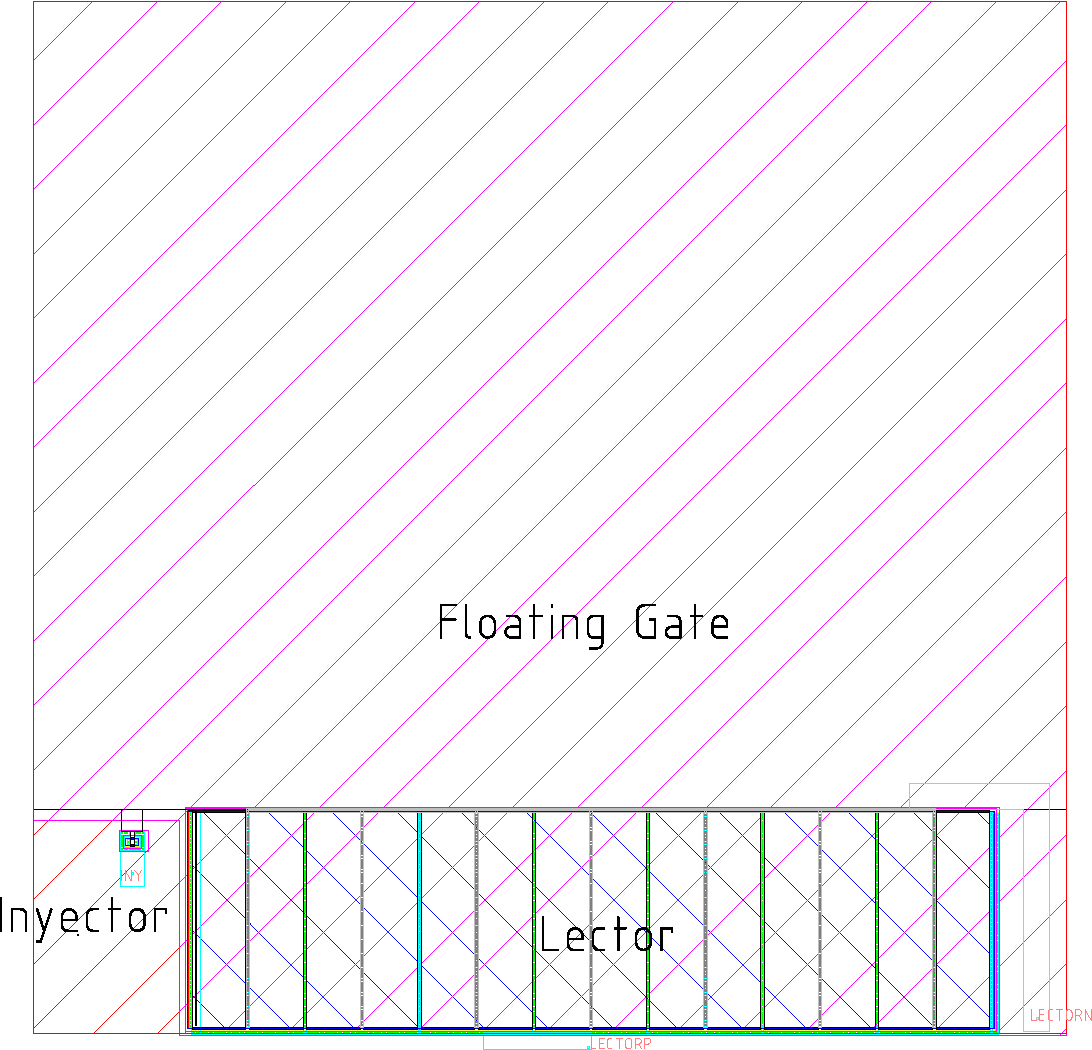
\includegraphics[width=\columnwidth]{figuras/aps/layout_hatch.pdf}
    \caption{Layout del dosímetro APS. 
    I1 es el espejo de corriente que polariza al primer seguidor M2.
    El transistor de reset M1 está conectado a un pad a través del
    circuito de protección de la \figref{fig:proteccion5v}.}
    \label{fig:layoutaps}
\end{figure}
\fig{proteccion5v}{figuras/aps/proteccion.pdf}
{Circuito de protección para la entrada de reset.
Los diodos sólo conducen si la tensión del pad excede \SI{5}{\volt} o
baja de \SI{0}{\volt}.
Esto evita que se polaricen en directa junturas del circuito que deben
permanecer en inversa (drain-bulk y source-bulk).}
La topología del circuito quedó determinada por la elección de construir un
dosímetro APS con un par de seguidores para su medición.
El paso siguiente en el diseño fue elegir los tamaños de los distintos
componentes para optimizar el desempeño del sensor (\figref{fig:falltime}).
\fig{falltime}{figuras/aps/falltime.pdf}
{Tiempo de respuesta simulado del buffer en función del W del transistor
final.}

Para una carga dada, la tensión sobre un capacitor es inversamente proporcional
a su capacidad.
Por lo tanto, maximizamos la señal producida por la radiación 
reduciendo las capacidades parásitas del cátodo de D1.
Para esto usamos transistores de área mínima en M1 y M2.
Restringimos el largo de las conexiones del cátodo,
y las mantuvimos alejadas de otros nodos.
Aplicamos software de Mentor de extracción de capacidades parásitas al layout
resultante, y obtuvimos una capacidad total en el cátodo de \SI{3.4}{\femto\farad}.
\begin{table}[h]
    \centering
    \caption{Dimensiones del diseño optimizadas para sensibilidad y tiempo de
    respuesta}
    \begin{tabular}{|c|c|}
        \hline
        Dispositivo&      Dimensiones\\
        \hline
D1&     \SI{4x4}{\micro\meter}\\
M1&     \SI{0.8x0.6}{\micro\meter}\\
M2&     \SI{0.8x0.6}{\micro\meter}\\
M3&     TODO\\
        \hline
    \end{tabular}
    \label{fig:areas}
\end{table}

Estas dimensiones se utilizaron tanto para la simulación del circuito en SPICE
como para los cálculos Monte-Carlo.
La combinación de estas dos herramientas nos da una sensibilidad esperada de 
\SI{7.1}{\volt\per\gray}.
\subsection{Medición}
Tomamos dos dies y los bondeamos a placas adaptadoras de TSSOP28,
un empaquetado de circuitos integrados de montaje superficial
(figuras~\ref{fig:bondeados1}, \ref{fig:bondeados2} y~\ref{fig:pinout}).
\fig{bondeados1}{figuras/aps/bondeados.jpg}
{Dies bondeados a placa adaptadora SMD.
Los zócalos tienen las patas cortocircuitadas para proteger al die de
descargas electrostáticas durante el transporte y almacenamiento.}
\figp{bondeados2}{figuras/aps/die.jpg}
{Detalle del die fabricado con los dosímetros APS y FG 
(arriba en la columna central)
y otros circuitos.}
\figp{pinout}{figuras/aps/pinout1.pdf}
{Layout del die entero con numeración de los pads bondeados}
\subsubsection{Descarga en oscuridad}
Primero medimos la respuesta del sensor sin luz ni radiación
(figuras~\ref{fig:oscuridad4} y~\ref{fig:oscuridad40}).
\fig{oscuridad4}{figuras/aps/oscuridad4.pdf}
{Curva de descarga en oscuridad del APS de 4x\SI{4}{\micro\meter}.
Resulta de resetear el APS y medir su tensión de salida en oscuridad.}
\fig{oscuridad40}{figuras/aps/oscuridad40.pdf}
{Curva de descarga en oscuridad del APS de 40x\SI{40}{\micro\meter}.
Resulta de resetear el APS y medir su tensión de salida en oscuridad.}
Esto nos muestra la descarga del diodo debido a la corriente de fuga en
inversa.

Se ve en ambas figuras la misma curva 
con escalas distintas de tiempo y de tensión.
Esta variación proviene tanto de las áreas distintas de los dos sensores
como del mismatching entre los seguidores.
Ya que éstos usan varios transistores de área mínima,
son particularmente sensibles a variaciones del proceso
(el mismo error absoluto en las dimensiones del canal produce un mayor error relativo).

% Descarga debería ser lineal
% https://books.google.com.ar/books?id=6Rg7AAAAQBAJ&lpg=PA289&ots=yO1HPv_N4E&dq=reverse%20biased%20diode%20%22discharge%20curve%22&hl=es&pg=PA290#v=onepage&q=reverse%20biased%20diode%20%22discharge%20curve%22&f=false
La forma de la curva proviene de la variación 
tanto de la corriente de fuga como de la capacidad del diodo.
Ambas dependen de la tensión aplicada,
debido a la variación del ancho de la zona desierta.
Al caer la tensión en inversa,
se vuelve más angosta.
Esto reduce su volúmen y por lo tanto 
la tasa de generación térmica de pares electrón-hueco.
Por otra parte,
su capacidad es inversamente proporcional a este ancho.
Ambos fenómenos reducen la tasa de descarga,
como se ve al final de ambas curvas.
%
\subsection{Iluminación con LED}
Medimos las curvas de descarga iluminando los dies con un LED,
variando su corriente para lograr distintas intensidades de iluminación
(figuras~\ref{fig:led4} y~\ref{fig:led40}).
\fig{led4}{figuras/aps/descarga_led_4.pdf}
{Curva de descarga iluminando con un LED el APS de 4x\SI{4}{\micro\meter}.
La corriente del LED aumenta de \SI{.1}{\milli\ampere} a la derecha hasta
\SI{10}{\milli\ampere} a la izquierda,
con 6 curvas por década.}
\fig{led40}{figuras/aps/descarga_led_40.pdf}
{Curva de descarga iluminando con un LED el APS de 40x\SI{40}{\micro\meter}.
La corriente del LED aumenta de \SI{.1}{\milli\ampere} a la derecha hasta
\SI{10}{\milli\ampere} a la izquierda,
con 6 curvas por década.}
Esto permite observar la compresión de la curva de descarga 
con el aumento de la radiación incidente.
\subsubsection{Ruido medido}
Establecimos que una medición con este dosímetro consiste en promediar 10
muestras de tensión.
Esto nos permite definir de manera precisa el ruido como la desviación estándar
de ese promedio.
Calculamos esa desviación estándar en base a las curvas medidas (figuras~\ref{fig:ruido4} 
y~\ref{fig:ruido40}).
\fig{ruido4}{figuras/aps/ruido4.pdf}{Ruido a la salida del APS de
    \SI{4x4}{\micro\meter}, calculado tomando diferencias entre muestras y
escalando para que represente el ruido en un promedio de 10 valores.}
\fig{ruido40}{figuras/aps/ruido40.pdf}{Ruido a la salida del APS de
    \SI{40x40}{\micro\meter}, calculado tomando diferencias entre muestras y
escalando para que represente el ruido en un promedio de 10 valores.}
Podemos convertir estos valores de ruido en dosis usando la sensibilidad
calculada.
Así llegamos a una resolución de \SI{2.0}{\milli\gray} y \SI{2.3}{\milli\gray}
para el APS de \SI{4x4}{\micro\meter} y \SI{40x40}{\micro\meter},
    respectivamente.
% TODO: completar con cálculos de sensibilidad/resolución y mediciones
